%%%%%%%%%%%%%%%%%%%%%%%%%%%%%%%%%%%%%%%%%
% Journal Article
% LaTeX Template
% Version 2.0 (February 7, 2023)
%
% This template originates from:
% https://www.LaTeXTemplates.com
%
% Author:
% Vel (vel@latextemplates.com)
%
% License:
% CC BY-NC-SA 4.0 (https://creativecommons.org/licenses/by-nc-sa/4.0/)
%
% NOTE: The bibliography needs to be compiled using the biber engine.
%
%%%%%%%%%%%%%%%%%%%%%%%%%%%%%%%%%%%%%%%%%

%----------------------------------------------------------------------------------------
%	PACKAGES AND OTHER DOCUMENT CONFIGURATIONS
%----------------------------------------------------------------------------------------

\documentclass[
	a4paper, % Paper size, use either a4paper or letterpaper
	10pt, % Default font size, can also use 11pt or 12pt, although this is not recommended
	unnumberedsections, % Comment to enable section numbering
	twoside, % Two side traditional mode where headers and footers change between odd and even pages, comment this option to make them fixed
]{LTJournalArticle}

% \addbibresource{sample.bib} % BibLaTeX bibliography file

\runninghead{} % A shortened article title to appear in the running head, leave this command empty for no running head

\setcounter{page}{1} % The page number of the first page, set this to a higher number if the article is to be part of an issue or larger work

% \usepackage[french, french]{babel}
% \frenchbsetup{StandardItemLabels=true}
% \usepackage{csquotes}

%----------------------------------------------------------------------------------------
%	TITLE SECTION
%----------------------------------------------------------------------------------------

\title{FEATURE} % Article title, use manual lines breaks (\\) to beautify the layout

% Authors are listed in a comma-separated list with superscript numbers indicating affiliations
% \thanks{} is used for any text that should be placed in a footnote on the first page, such as the corresponding author's email, journal acceptance dates, a copyright/license notice, keywords, etc
\author{%
	Wagner Nicolas\thanks{Auteur correspondant: \href{mailto:nicolas@feature.sh}{nicolas@feature.sh}\\ \textbf{Publié le:} 6 Décembre 2023}
}

% Full-width abstract
\renewcommand{\maketitlehookd}{%
    \begin{abstract}
        \noindent FEATURE redéfinit l'engagement dans le développement
        \emph{open-source} en intégrant des \emph{crypto-rewards} aux tâches de
        développement sur GitHub. Cette approche fournit les conditions
        nécessaires pour inciter les développeurs à s'investir
        pleinement dans leurs contributions, tout en garantissant un livrable de
        qualité. L'\emph{Atomic Contract} de FEATURE facilite
        des transactions sécurisées et transparentes, offrant une rémunération
        claire et directe pour les développeurs. Ainsi, FEATURE transforme la
        collaboration \emph{open-source} en une expérience simple et gratifiante,
        accélérant l'évolution de l'écosystème
        du développement logiciel \emph{Open Source}.
    \end{abstract}
}

%----------------------------------------------------------------------------------------

\begin{document}

\maketitle % Output the title section

%----------------------------------------------------------------------------------------
%	ARTICLE CONTENTS
%----------------------------------------------------------------------------------------

\section{Introduction}

Depuis l'avènement d'Internet, les procédés de travail ont radicalement changé, passant de méthodes bien souvent localisées, individuelles et manuelles à des approches globales, collaboratives et numériquement connectées. Les e-mails, les forums de discussions et les premiers sites web ont considérablement participé à
la généralisation du travail collaboratif. L'une des avancées les plus significatives de ces outils est la possibilité de communiquer et de partager des informations de manière instantané à l'échelle mondiale, favorisant l'essor du travail à distance et du travail indépendant.

Les professionnels ont commencé à exploiter ces nouvelles opportunités pour proposer leurs compétences et leurs services à un public mondial. En parallèle, les modes de rémunération ont fortement évolué. Le traditionnel salariat s'est vu fortement concurrencé par le paiement à l'heure, au projet et même à la tâche (\emph{microtasking})..

Cette évolution des modèles engendre, d'une part, une concurrence plus importante qui profite aux recruteurs mais d'un autre côté permet aux indépendants d'avoir un accès à une offre de missions plus importantes et plus diversifiés. Pour répondre à ce besoin de mettre en relation clients et \emph{freelancers}, de nombreuses \emph{marketplace} de \emph{freelancing} ont vu le jour comme par exemple \emph{Upwork} ou \emph{Fiverr}.

Ces plateformes s'adaptent aux besoins changeants du marché du travail. Elles peuvent offrir des fonctionnalités avancées telles que des systèmes de notation, des outils de gestion de projet et des services de suivi du travail en cours. Les dernières tendances et technologies de ces dernières années telles que l'intelligence artificielle et la blockchain poussent certaines de ces plateformes à innover pour offrir un service toujours plus attractif.

FEATURE se positionne à l'avant-garde de cette transformation. En intégrant des \emph{smart contracts} blockchain avec des \emph{crypto-rewards} directement sur GitHub, FEATURE offre une couche d'incitation économique sur un outil sur lequelles développeurs ont l'habitude de travailler. La récompense des tâches de développement en crypto-monnaies via Github, assure des transactions sécurisées et transparentes propulsant l'innovation collaborative vers de nouveaux horizons.

%------------------------------------------------

\section{GitHub, \emph{Open-Source}, and FEATURE}

Github est initialement une solution d'hébergement et de suivi de version du code avec une interface web. L'interface graphique montre les diverses évolutions du code réalisé par le logiciel Git. Github a évolué pour offrir tout un panel d'outils autour du code comme le suivi de tâche (\emph{issue tracking}), la gestion de projet (Github Project), la partie devOps (Github Actions) ainsi que la possibilité aux applications tierces de s'intégrer à cet écosystème grâce aux "extensions" Github.

FEATURE s'appuie sur cette fonctionnalité d'extension Github. Elle est d'ailleurs listée sur la Marketplace Github. L'intégration Github permet une gestion simplifiée des \emph{crypto-rewards}. Il n'est pas nécessaire de passer par une application tierce pour pouvoir l'utiliser. La création, la réclamation et le paiement du \emph{crypto-reward} se font directement sur Github. Ce qui présente deux avantages majeurs:
\begin{itemize}
\item
  le premier pour le client, puisque le crypto-reward étant directement sur Github, le client touche les développeurs où ils sont déjà. Ce qui augmente le pouvoir d'attirer un plus grand nombre de développeurs.
\item
  le second pour les développeurs, leur mode de travail s'en trouve simplifié puisqu'il se passe sur une plateforme sur laquelle ils ont l'habitude de travailler.
\end{itemize}

La plateforme Github a largement contribué à l'\emph{Open Source} dans son ensemble et en particulier dans le domaine de la blockchain. \emph{Bitcoin} et \emph{Ethereum} en sont des exemples parmi tant d'autres. L'\emph{Open Source}, qui fait référence aux logiciels où le code est accessible à tous, attire de nombreux développeurs mais c'est bien souvent un "marché" non lucratif. Pour ces derniers, les motivations peuvent être diverses: technique (monter en compétence, résoudre un \emph{bug} pour utiliser le programme\ldots), social (se construire un \emph{portfolio} de contributions) et économique (récompense donnée pour avoir trouvé une faille de sécurité\ldots). Cependant, bien souvent, ces facteurs ne suffisent pas à stimuler une participation massive des développeurs externes. Cela est encore plus vrai quand il s'agit de réaliser des contributions majeures, ces dernières étant le fruit d'un groupe restreint de développeurs rémunérés par une fondation
ou un organisme privé.

Alors, comment activer davantage les contributions externes?

L'hypothèse de FEATURE est que même s'il existe des raisons pour contribuer à un projet \emph{Open Source} (technique, social\ldots), ce n'est seulement que par des incitations économiques systémiques et directement sur Github que l'on peut considérablement augmenter le nombre de contributions majeures de la part de la communauté des développeurs.

Ainsi, FEATURE se positionne sur ce marché du \emph{freelancing} dans le domaine du développement en associant à chaque tâche Github (\emph{Issue}) un \emph{crypto-reward} avec pour objectif d'activer davantage les contributeurs et de ce fait, accélérer l'écosystème \emph{Open Source}.

%------------------------------------------------

\section{Atomic Contract}

L'idée d'effectuer des paiements en crypto-monnaie est née en 2008 avec la publication du livre blanc "Bitcoin". La crypto-monnaie permet d'effectuer des transactions de pair à pair de manière sécurisée, sans l'intervention d'une tiers de confiance. Cela signifie que les utilisateurs peuvent effectuer des paiements directement les uns aux autres, sans faire recours à un intermédiaire pour valider ou vérifier les transactions.

Ce concept a été étendu à la création de \emph{smart contract} qui permet à des utilisateurs ou programmes d'interagir avec des programmes qui exécutent "automatiquement" des actions prédéfinies lorsque des conditions spécifiques sont remplies.

Enfin, ces \emph{smart contrats} peuvent être particulièrement utiles pour réaliser des mises sous séquestre où des fonds provisionnés seront libérés que sous certaines conditions définies par le \emph{smart contract}. Ce type particulier de programmes sont appelés les \emph{Escrow Smart Contract}.

L'\emph{Atomic Contrat} concilie ces différents concepts, cryptomonnaies, \emph{smart contract} et mise sous séquestre pour réaliser des transactions économiques sous certaines conditions (\emph{contract}) et spécifique à une tâche (\emph{atomic}).

L'intérêt de celui-ci dans le domaine du \emph{freelance} est de pouvoir passer d'une rémunération au temps, comme dans le salariat par exemple, ou au projet, proposé souvent par des agences, à une rémunération à la tâche. Les tâches de développement sont particulièrement bien géré sur Github via les \emph{issues}. Les \emph{issues} Github permettent de décrire la tâche avec un fil de discussion pour suivre son évolution et laisser des remarques si nécessaires. FEATURE ajoute à ces \emph{issues} directement dans le fil de discussion un \emph{crypto-reward} pour inciter les développeurs à réaliser la tâche. La rémunération associée à la tâche est libérée que si les conditions ont été respectées, que sont le délai de livraison et la qualité du livrable. C'est en ceci que FEATURE propose des \emph{Atomic Contracts}.

Rémunérer à la tâche permet de sortir d'un système de rémunération assez flou qu'est la rémunération au projet ou au temps. En effet, comment calculer rétrospectivement la valeur qu'a apportée chaque développeur au projet alors que la livraison de celui-ci peut survenir plusieurs semaines ou mois après les premiers développements ? Cela peut s'avérer très compliqué d'autant plus s'il n'y pas un suivi régulier des contributions.

En s'appuyant sur les \emph{Atomic Contracts}, FEATURE assure les transactions économiques client-développeur ce qui donne plus confiance au développeur d'investir du temps pour réaliser la tâche et pour le client, de gérer les coûts de développement de manière plus précise.

%------------------------------------------------

\section{Configuration}

FEATURE offre plusieurs types de configuration pour s'adapter au mieux aux besoins des utilisateurs que ce soit en termes d'expérience utilisateur ou de sécurité. Pour répondre au mieux aux besoins de l'utilisateur, il est possible de configurer:

\begin{itemize}
\item
  le montant de la transaction que ce soit en \emph{coin} (\emph{token} native d'une blockchain) ou en \emph{token} qui suit le standard ERC20.
\item
  et le délai dans lequel doit être réalisé la tâche.
\end{itemize}

\begin{figure*}[ht]
  \centering
  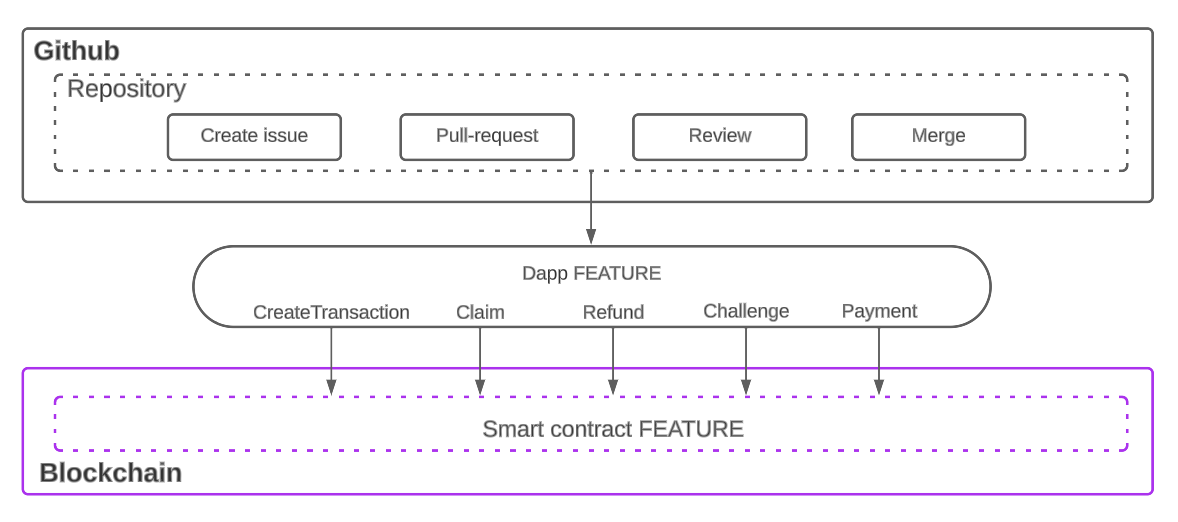
\includegraphics[width=0.95\textwidth]{media/diagram_web3_Feature.png}
  \caption{Diagramme web3 FEATURE - Ce schéma représente une vue d'ensemble de flux de travail de la Dapp FEATURE, utilisant la gestion du code provenant des répertoires Github aux interactions avec les smart contracts de la blockchain.}
  \label{fig:web3 diagram}
\end{figure*}

En plus de cette configuration de base, il est possible de configurer les incitations économiques pour assurer la qualité du livrable:

\begin{itemize}
\item
  le temps de \emph{challenge} pendant lequel des \emph{reviewers} vont pouvoir \emph{challenger} le développeur qui a réalisé la tâche,
\item
  un \emph{deposit} réalisé au moment de la proposition de code du développeur pour inciter d'autres développeurs à faire la revue de son code,
\item
  et enfin l'arbitre pour résoudre la dispute entre l'\emph{issuer} et le \emph{challenger} en cas de litige, cela peut-être un arbitre centralisé, une multisig ou une DAO (Kleros).
\end{itemize}

En plus de ces configurations, il est possible d'effectuer les transactions en mode \emph{self-custodial} ou \emph{custodial}. L'avantage du mode custodial est de ne plus se soucier des transactions blockchains. Il se configure simplement en provisionnant un \emph{wallet} et en associant à chaque label Github, qui permet de base de \emph{tagger} les \emph{issues} par exemple la difficulté de l'issue, à un \emph{Atomic Contract}. Ce mode assure une expérience extrêmement fluide puisque les \emph{Atomic Contracts} seront alors automatiquement créés au moment de la labellisation d'une \emph{issue}. Ce dernier mode, concilie l'avantage des \emph{Atomic Contracts} avec une "expérience web2" bien plus fluide pour les utilisateurs.

%------------------------------------------------

\section{Workflow}

Voyons l'expérience utilisateur en décrivant étapes par étapes le workflow de la création de l'\emph{Atomic Contract} à sa conclusion c'est-a-dire son paiement ou éventuellement sa résolution via l'arbitre:

\begin{enumerate}
\def\labelenumi{\arabic{enumi}.}
\item
  création de l'\emph{issue} Github;
\item
  étiquetage de l'issue avec label Github configuré avec FEATURE pour générer l'\emph{Atomic Contract} et mettre sous séquestre le \emph{crypto-reward};
\item
  discussion sur le travail à faire, voire en cours, directement dans le fil de discussion de l'\emph{issue}, et le remboursement des fonds pour l'\emph{issuer} dans le cas où il n'y pas eu de propositions de code, appelé \emph{pull-request}, dans le temps imparti;
\item
  création d'une \emph{pull-request} par un développeur et enregistrement de cette proposition sur l'\emph{Atomic Contract};
\item
  revue du code par des développeurs et éventuellement soumission d'une dispute si jamais le \emph{challenger} pense que les spécificités n'ont pas été respectés;
\item
  dans le cas d'une dispute, soit le \emph{challenger} percevra le \emph{deposit} du développeur et l'\emph{Atomic Contract} sera disponible pour accepter de nouvelles propositions de code, soit le développeur gagne la dispute, il gagnera alors le \emph{crypto-reward} et l'\emph{Atomic Contract} sera terminé;
\item
  le \emph{merge} de la \emph{pull-request} afin d'ajouter l'implémentation de la solution proposée sur la source principale du code.
\end{enumerate}

Le diagramme Figure \ref{fig:web3 diagram} récapitule ces différentes étapes.

Ce workflow assure une expérience optimale aussi bien pour le développeur, en lui proposant une expérience aussi proche de ce qu'il a l'habitude de faire sur Github avec l'assurance d'être payé s'il respecte les spécificités décrites dans l'issue, que pour l'\emph{issuer} qui grâce au système de \emph{review} peut s'assurer d'un livrable de qualité fournit dans le temps imparti, qui dans le cas où ces exigences ne sont pas respectés se verra remboursé.

\section{Conclusion}

FEATURE offre un outil simple pour inciter les développeurs à contribuer aux projets \emph{Open-Source} avec des \emph{crypto-rewards}. Cette incitation se fait via la création d'un \emph{Atomic Contract} pour assurer d'une part au développeur d'être payé et l'\emph{issuer} que le livrable est de qualité et fournit dans le temps imparti.

L'expérience pour le développeur est au plus proche de ce qu'il a l'habitude de faire aussi bien pour consulter les tâches à réaliser, que pour réaliser des revues de code et éventuellement recevoir les \emph{crypto-rewards} pour ce travail. Pour l'\emph{issuer}, réaliser les offres directement sur Github et de manière automatique via les labels Github va lui permettre de toucher les développeurs où ils sont déjà et simplifier la création d'offres.

Grâce à FEATURE, la collaboration sur Github n'aura jamais été aussi simple et gratifiante, ce qui en fait un outil idéal pour accélérer le développement de code des projets \emph{Open-Source}.

\end{document}
